\subsection{RMW Layer Structures}
% - NOTE: -------------------------------------------------------------
\subsubsection{WORKING: wait}
\textbf{1. \str{rmw\_wait\_set\_t}}: Container for guard conditions to be waited on.
\begin{figure}[htbp!]
    \centering
    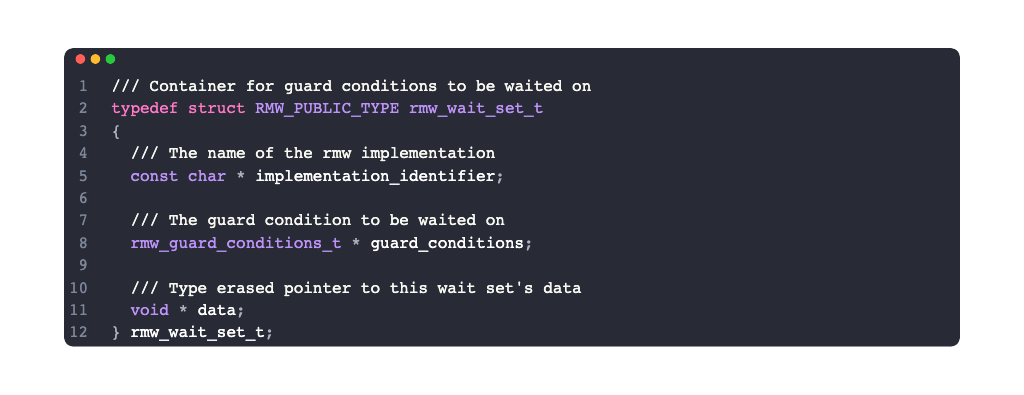
\includegraphics[width=1\linewidth]{Sec/Implementation/rmw/fig/rmw_wait_set_t.png}
    \caption{Structure: rmw\_wait\_set\_t}
    \vspace{-0.1in}
\end{figure}

\textbf{2. \str{rmw\_guard\_conditions\_t}}: Array of guard condition handles. An array of void * pointers representing type-erased middleware-specific guard conditions. The number of non-null entries may be smaller than the allocated size of the array. The number of guard conditions represented may be smaller than the allocated size of the array. The creator of this structure is responsible for allocating and de-allocating the array.
\begin{figure}[htbp!]
    \centering
    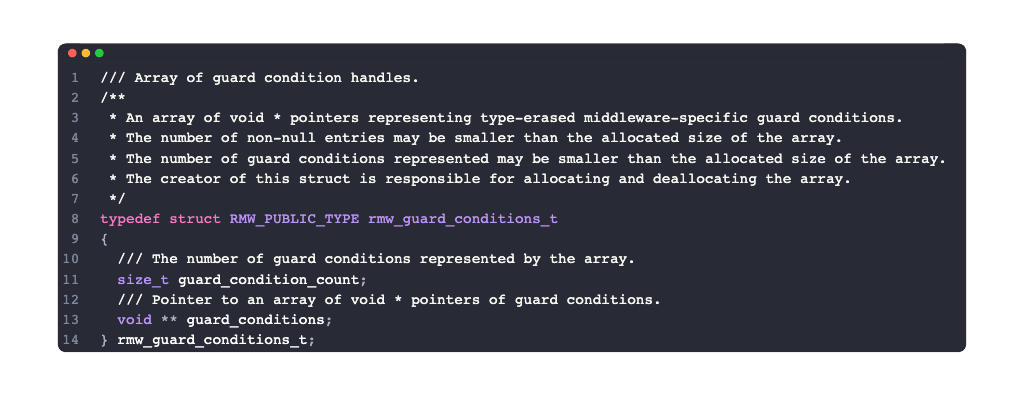
\includegraphics[width=1\linewidth]{Sec/Implementation/rmw/fig/rmw_guard_conditions_t.png}
    \caption{Structure: rmw\_guard\_conditions\_t}
    \vspace{-0.1in}
\end{figure}